\documentclass[12pt,preprint]{aastex}
% for \sout
\usepackage{ulem}
% makes sure \em{} is italic rather than underlined (corrects ulem from line above)
\normalem

% for the red MarginPars
\usepackage{color}

% some extra math symbols
\usepackage{mathtools}

% allows Greek symbols to be bold
\usepackage{bm}

\newcommand{\rhocutoff}{\rho_\mathrm{cutoff}}
\newcommand{\rhoanelastic}{\rho_\mathrm{anelastic}}

\newcommand{\gcc}{\mathrm{g~cm^{-3} }}
\newcommand{\Tcutoff}{T_\mathrm{cutoff}}

% MarginPars
\setlength{\marginparwidth}{0.75in}
\newcommand{\MarginPar}[1]{\marginpar{\vskip-\baselineskip\raggedright\tiny\sffamily\hrule\smallskip{\color{red}#1}\par\smallskip\hrule}}


\newcommand{\evm}{{(-)}}
\newcommand{\evz}{{(\circ)}}
\newcommand{\evp}{{(+)}}
\newcommand{\enu}{{(\nu)}}



\newcommand{\msolar}{\mathrm{M}_\odot}

\begin{document}

%==========================================================================
% Title
%==========================================================================
\title{Double White Dwarf Mergers with CASTRO\\ I. Methodology and Code 
       Verification}

\shorttitle{DWD Mergers. I. Methodology}
\shortauthors{Max}

\author{TBD}
%==========================================================================
% Abstract
%==========================================================================
\begin{abstract}
We describe our numerical methodology for modeling double white dwarf
systems with the AMR hydrodynamics code Castro.

\end{abstract}
\keywords{hydrodynamics - methods: numerical - supernovae: general - white dwarfs}

%==========================================================================
% Introduction
%==========================================================================
\section{Introduction}

Type Ia supernovae (SNe Ia) are currently some of the most exciting events to study in astrophysics. These bright, brief pulses of light in the distant universe have led to a number of important discoveries in recent years, including the discovery of the accelerated expansion of the universe \citep{perlmutter1999,riess1998}. However, their origin is shrouded in mystery. It has long been expected that these events arise from the thermonuclear explosions of white dwarfs \citep{hoyle_fowler:1960}, but the cause of these explosions is uncertain. In particular, it is not clear what process causes the temperatures in these white dwarfs to become hot enough for explosive burning of its constituent nuclei. The model favored initially by the community was the so-called single-degenerate (SD) model. Accretion of material from a companion star such as a red giant would cause the star to approach the Chandrasekhar mass, and in doing so the temperature and density in the center would become sufficient for thermonuclear fusion to proceed. A review of the observational evidence and theoretical modelling that formed this belief can be found in \citet{hillebrandtniemeyer2000}.


%==========================================================================
% Numerical Methodology
%==========================================================================
\section{Numerical Methodology}\label{sec:Numerical Methodology}

\subsection{Hydrodynamics}

We use the unsplit PPM solver in Castro to advance the hydrodynamics
system in time.  A number of changes were made to the solver, which are 
detailed in the Appendix.  These changes bring the algorithm more in 
line with that of \cite{ppm}.  

The boundary conditions on the hyperbolic system are simply
zero-gradient.  Using AMR, we make the coarse grid very large, so as
to place the boundaries far from the region of interest.  We further
make the restriction that only level-0 (coarse) grids can touch the
domain boundary.



AMR

rotation


\subsection{Microphysics}

The equation of state (EOS) for our simulations is the Helmholtz EOS \citep{timmes_swesty:2000}. This models an electron-positron gas of arbitrary relativity and degeneracy over a wide range of temperatures and densities. Thermodynamic quantities are calculated as derivatives of the Helmholtz free energy, and the values are interpolated from a table. The natural variables of the Helmholtz free energy are temperature and density, and calling the EOS is simplest in this form. However, in hydrodynamics we often have the density, and internal energy as independent variables, and we want to obtain the temperature, pressure, and other quantities. To do this, we employ a Newton-Raphson iteration over the temperature (given some sufficient starting guess) until we find the temperature that corresponds to the desired internal energy. Sometimes this process fails to converge and the iterative value approaches zero. In these cases we employ a ``floor'' that limits how low the temperature can go (typically $10^4$ or $10^5$ K). There is a choice here how to proceed: we can either assign this floor value to the temperature and let that zone be thermodynamically inconsistent (the original behavior in Castro), or we can adjust the internal energy to be thermodynamically consistent with the temperature, at the cost of violating energy conservation. We have found in test problems of one-dimensional shocks that the latter yields more accurate results, so we employ the latter method.

Reactions?

\subsection{Initial Models}
\label{sec:initial_models}

We generate initial models by integrating the equation of hydrostatic
equilibrium, taking the temperature and composition to be constant,
and using the general stellar equation of state.  This results in
a single nonlinear equation to find the density in a zone given the
conditions in the zone beneath it:
\begin{equation}
\frac{p(\rho_{i+1}) - p_i}{\Delta x} = \frac{1}{2} (\rho_i + \rho_{i+1}) g_{i+1/2}
\end{equation}
This is solved via Newton iteration to give $\rho_{i+1}$.  Here, $g_{i+1/2}$
is the gravitational acceleration at the interface between zones $i$ and $i+1$,
found by simply adding up all the mass from zones $1, \ldots, i$ to get the
enclosed mass, $M_{i+1/2}$, and then $g_{i+1/2} = -GM_{i+1/2}/r_{i+1/2}^2$.

To start the integration off, we need a central density.  We guess at
this, and then iterate over the entire integration procedure to find
the central density needed to yield the desired total mass.  Finally,
we generate the initial model at the same resolution as the finest
grid in our simulation.

We map the 1-d model onto the 3-d Cartesian grid by taking density,
temperature, and composition as the independent variables,
interpolating these to the cell-centers, and then calling the equation
of state to initialize the remaining terms.  The velocity is taken to
be zero in the rotating frame initially.

\subsection{Gravity}

We solve the Poisson equation for self-gravity for our problem,
\begin{equation}
  \nabla^2 \Phi(\mathbf{x}) = -4\pi G\, \rho(\mathbf{x}),
\end{equation}
where $\Phi$ is the gravitational potential, $G$ is the gravitational constant, and $\rho$ is the mass density. We note that the sign convention used in CASTRO is opposite to that commonly seen in the physics literature, so that $\Phi$ is positive everywhere. The solution of this equation in CASTRO is described in \cite{castro}, and consists of both level and composite solves, and a final synchronization at the end.

Analytic solutions to the Poisson equation customarily assume that the potential vanishes at large distances from the region of non-zero density. However, on a finite computational domain it is usually not possible to have the edges of the domain be far enough away that the potential can be taken to be zero there. Solving the Poisson equation therefore requires knowledge of the values of the potential on the edges of the computational domain. In principle, they can be computed by doing a direct sum over the mass distribution inside the domain, where the mass in each zone is treated as a point source:
\begin{equation}
  \Phi_{\text{lmn}} = G\, \sum_{\text{i, j, k}} \frac{G \rho_{\text{ijk}}}{|\mathbf{x}_{\text{lmn}} - \mathbf{x}_{\text{ijk}}|}\, \Delta V_{\text{ijk}}.\label{direct_sum}
\end{equation}
Here (i, j, k) are the indices of cells inside the domain, and (l, m, n) are the indices of boundary locations. $\Delta V$ is the volume of the zone. We have implemented this as an option\footnote{It is controlled with the \texttt{gravity.direct\_sum\_bcs} input parameter.} in CASTRO. If there are $N$ zones per spatial dimension, then there are $6 N^2$ boundary zones, and each boundary zone requires a sum over $N^3$ zones, so the direct computation of the boundary conditions scales as $N^5$.  This method is expensive enough that it is not used for hydrodynamics simulations (though it is useful for comparison to the approximate solutions described below).

In a typical simulation we place the boundaries of the domain far enough away from the region containing most of the mass that some method of approximation to this direct summation is justified. Many approaches exist in the literature. The original release of CASTRO featured the crudest possible approximation: a monopole prescription, where the boundary values were computed by summing up all the mass on the domain and treating it as a point source at the domain center. This is exactly correct only for a spherically symmetric mass distribution, and indeed this is often a sufficient approximation for single-star Type Ia supernova simulations that employ self-gravity (ref). However, for a problem like that of a binary star system with significant departures from spherical symmetry, this assumption fails to produce accurate boundary values. This results in a significant drift of the center of the mass of the system over time. We describe here two new features we have added to CASTRO to address this issue.

\subsubsection{Multipole Expansion}

The most natural extension of the monopole prescription is to include higher-order multipole moments. If the entire mass distribution is enclosed, then the potential can be expanded in a series of spherical harmonics $Y_{lm}$:
\begin{equation}
  \Phi(\mathbf{x}) = \sum_{l=0}^{\infty}\sum_{m=-l}^{l} \frac{4\pi}{2l + 1} q_{lm} \frac{Y_{lm}(\theta,\phi)}{r^{l+1}}, \label{spherical_harmonic_expansion}
\end{equation}
where $q_{lm}$ are the so-called multipole moments. The origin of the coordinate system is taken to be the center of the computational domain, and $r$ is the distance to the origin. The multipole moments can be calculated by expanding the Green's function for the Poisson equation as a series of spherical harmonics.
\begin{comment}
, which yields
\begin{equation}
  q_{lm} = \int Y^*_{lm}(\theta^\prime, \phi^\prime)\, {r^\prime}^l \rho(\mathbf{x}^\prime)\, d^3x^\prime. \label{multipole_moments_original}
\end{equation}
\end{comment}
After some algebraic simplification of Equation \ref{spherical_harmonic_expansion} using the addition theorem for spherical harmonics,
\begin{comment}
\begin{align}
  &\frac{4\pi}{2l+1} \sum_{m=-l}^{l} Y^*_{lm}(\theta^\prime,\phi^\prime)\, Y_{lm}(\theta, \phi) = P_l(\text{cos}\, \theta) P_l(\text{cos}\, \theta^\prime) \notag \\
  &\ \ + 2 \sum_{m=1}^{l} \frac{(l-m)!}{(l+m)!} P_{l}^{m}(\text{cos}\, \theta)\, P_{l}^{m}(\text{cos}\, \theta^\prime)\, \left[\text{cos}(m\phi)\, \text{cos}(m\phi^\prime) + \text{sin}(m\phi)\, \text{sin}(m\phi^\prime)\right].
\end{align}
\end{comment}
the potential outside of the mass distribution can be written as:
\begin{equation}
  \Phi(\mathbf{x}) = \sum_{l=0}^{\infty} \left[Q_l^{(0)} \frac{P_l(\text{cos}\, \theta)}{r^{l+1}} + \sum_{m = 1}^{l}\left[ Q_{lm}^{(C)}\, \text{cos}(m\phi) + Q_{lm}^{(S)}\, \text{sin}(m\phi)\right] \frac{P_{l}^{m}(\text{cos}\, \theta)}{r^{l+1}} \right].\label{multipole_potential}
\end{equation}
$P_l(x)$ are the Legendre polynomials and $P_{l}^{m}(x)$ are the associated Legendre polynomials. $Q_l^{(0)}$ and $Q_{lm}^{(C,S)}$ are variants of the multipole moments that involve integrals of $P_l$ and $P_l^m$, respectively, over the computational domain.
\begin{comment}
\begin{align}
  Q_l^{(0)}   &= \int P_l(\text{cos}\, \theta^\prime)\, {r^{\prime}}^l \rho(\mathbf{x}^\prime)\, d^3 x^\prime \\
  Q_{lm}^{(C)} &= 2\frac{(l-m)!}{(l+m)!} \int P_{l}^{m}(\text{cos}\, \theta^\prime)\, \text{cos}(m\phi^\prime)\, {r^\prime}^l \rho(\mathbf{x}^\prime)\, d^3 x^\prime \\
  Q_{lm}^{(S)} &= 2\frac{(l-m)!}{(l+m)!} \int P_{l}^{m}(\text{cos}\, \theta^\prime)\, \text{sin}(m\phi^\prime)\, {r^\prime}^l \rho(\mathbf{x}^\prime)\, d^3 x^\prime.
\end{align}
\end{comment}
This approach becomes computationally feasible when we cut off the outer summation in Equation \ref{multipole_potential} at some finite value of $l_{\text{max}}$. If it is of sufficiently high order, we will accurately capture the distribution of mass on the grid. In practice we first evaluate the discretized analog of the modified multipole moments for $0 \leq l \leq l_{\text{max}}$ and $1 \leq m \leq l$, an operation that scales as $N^3$. We then directly compute the value of the potential on all of the $6N^2$ boundary zones. Since the multipole moments only need to be calculated once, the full operation scales only as $N^3$. The amount of time required to calculate the boundary conditions will be directly related to the chosen value of $l_{\text{max}}$, so there is a trade-off between computational expense and accuracy of the result. We find that for the early stages of the evolution of the binary system, $l_\text{max} \approx 6$ is sufficient.

\subsubsection{Isolated Potential}

%Figure~\ref{fig:2levgrav} shows the sequence of updates for $\phi$ on a 2-level grid.
A clever way to evaluate Equation \ref{direct_sum} exactly for the boundary values of the potential was described by \cite{james77}, and we have implemented a method inspired by that work here. In electrostatics a commonly encountered boundary-value problem is that of a positive charge distribution inside of a grounded conducting box. The potential vanishes on the surface of the box. For this to happen, a collection of negative charges must form on the outer surface of the box, to compensate the charge enclosed inside the box. This can be described by a surface charge density $\sigma$. This construction is useful in determining what the potential would be at the location of the surface when the box is removed. We will describe the potential outside of a density distribution that is non-zero only in some finite region as ``isolated'', and denote it by $\Phi$. This is the quantity we want to solve for. The potential in the case where the surface is grounded and conducting is called the ``homogeneous'' potential, and will be denoted by $\phi$. The homogeneous potential is the sum of the isolated potential and also the potential due to the surface charges $\Psi$:
\begin{equation*}
  \phi = \Phi + \Psi.
\end{equation*}
In order for $\phi$ to vanish at the surface, $\Phi$ and $\Psi$ must be of opposite sign, which makes sense since they are generated by opposite-sign charges. Rearranging this equation for the isolated potential yields
\begin{equation}
  \Phi = \phi - \Psi.
\end{equation}
Therefore a strategy for finding $\Phi$ is: solve the Poisson equation with homogeneous boundary conditions for $\phi$; calculate the necessary surface charges $\sigma$; find the resulting $\Psi$ on the boundary of the domain; solve the Laplace equation with inhomogeneous boundary conditions for $\Psi$ inside the domain; and then take $\Phi = \phi - \Psi$.

We slightly simplify this approach by observing that, since $\phi$ is by construction zero on the boundary, the value of $\Psi$ everywhere on the boundary must be equal in magnitude and opposite in sign to $\Phi$. Therefore the problem of finding the boundary values for $\Phi$ is reduced to solving the Poisson equation for $\phi$, constructing the surface charges $\sigma$, and then performing the appropriate integration of $-\sigma$ to get the boundary values. We then proceed with the Poisson solve as normal.

All of this can be done for the gravitational version of Poisson's equation. Even though we do not commonly speak of negative gravitational charges, they are simply a mathematical tool for obtaining the correct potential. In general,
\begin{equation}
  \sigma = \frac{1}{4\pi G} {\bm{\nabla}} \phi \cdot \hat{\mathbf{n}},\label{eq-isolated-sigma}
\end{equation}
where $\hat{\mathbf{n}}$ is the unit vector perpendicular to (and pointing away from) the surface. On the computational domain, using an appropriate discretized representation of the ${\bm{\nabla}}$ operator, we calculate $\sigma$ at every boundary location. This requires some care. In CASTRO, the boundaries are on cell edges a distance $dx / 2$ away from the outermost domain location. It is therefore tempting to use a central difference that uses the ghost zone on one side and the outermost zone inside the domain in the other. This is normally second-order accurate. However, by construction, the gradient of $\phi$ is discontinuous across that surface; it is zero just outside the surface, and non-zero just inside the surface. This discontinuity is what establishes the non-zero surface mass density, similar to how a jump in the electric field is associated with a surface charge density in electrostatics. Therefore it is inappropriate to use the central difference method. Instead, a one-sided difference is required, using only the data interior to the surface. For the discretization to be second-order accurate, data from the two nearest cells must be used. Generally, $\left.\partial f/\partial x\right|_{\rm i} = (-3 f_{\rm i} + 4 f_{\rm i+1} - f_{\rm i+2}) / (2 \Delta x)$ is a second-order accurate forward difference to the derivative of a function $f$ at zone index i; however, we are indexing from the domain edge, which does not coincide with a cell center. We can use this formula on our finite volume grid if we let $\Delta x \to \Delta x / 2$ (here we assume that the index 0 corresponds to the left-most cell center):
\begin{equation*}
  \left.\frac{\partial \phi}{\partial x}\right|_{-1/2} = \frac{-3 \phi_{-1/2} + 4 \phi_{0} - \phi_{1/2}}{2(\Delta x / 2)} + \mathcal{O}(\Delta x^2).
\end{equation*}
To proceed, we note that $\phi_{-1/2} = 0$ by construction, and $\phi_{1/2} = (\phi_{1} + \phi_{0}) / 2$ to second order, so:
\begin{equation}
  \left.\frac{\partial \phi}{\partial x}\right|_{-1/2} = \frac{7\phi_{0} - \phi_{1}}{2\Delta x} + \mathcal{O}(\Delta x^2).
\end{equation}
A similar formula holds for the one-sided (backward) difference at the opposite boundary. Once this gradient has been calculated, we can calculate surface masses using Equation \ref{eq-isolated-sigma} (recalling to negate the result to obtain positive masses, following the above discussion). For example, for a mass on the lower surface of constant $x$,
\begin{equation}
  M_{-1/2} = -\sigma_{-1/2} \Delta A = \frac{1}{4\pi G} \frac{7\phi_{0} - \phi_{1}}{2\Delta x}\Delta y \Delta z.
\end{equation}
According to Gauss' law, the total mass induced on the surface should be equal to the mass enclosed inside the boundary. We have verified directly that the sum of the mass added on the surface approaches the total mass inside the domain at a second-order rate of convergence.

We can then find the resulting potential on the boundary by summing over all of the surface charges:
\begin{equation}
  \Psi_{\text{l,m,n}} = \sum_{\text{l$^\prime$,m$^\prime$,n$^\prime$}} g_{\text{l-l$^\prime$},\text{m-m$^\prime$},\text{n-n$^\prime$}} M_{\text{l$^\prime$,m$^\prime$,n$^\prime$}}
%= \sum_{\text{l$^\prime$,m$^\prime$,n$^\prime$}} \frac{GM_{\text{l$^\prime$,m$^\prime$,n$^\prime$}}}{\left|\mathbf{x}_{\text{l,m,n}} - \mathbf{x}_{\text{l$^\prime$,m$^\prime$,n$^\prime$}}\right|}
\end{equation}
Here (l, m, n) refer only to boundary locations, and $g_{\text{a},\text{b},\text{c}}$ is the Green's function for the Poisson equation. At large distances, this is simply $G / r$, where $G$ is the gravitational constant and $r$ is the distance. However, this analytical expression is not correct for the discretized Laplacian, and the corresponding Green's function is a series in the odd powers of $1/r$. We use the expression derived by \citet{burkhart:1997}, only retaining the terms up to $r^{-5}$. Also, this expression nominally diverges at $r = 0$, which physically corresponds to the self-contribution to the potential from a zone. However, this singularity is integrable: the cell does have a contribution to its own potential. A numerical evaluation of the integral of the Green's function over a cubic region yields $\phi(r = 0) = 2.38\, G M / \Delta x$, assuming $\Delta x = \Delta y = \Delta z$, and so our Green's function at the origin is $g_{0,0,0} = 2.38\, G / \Delta x$. This is similar to how other authors treat this singularity, for example \citet{hockney_eastwood}. However, they simply set the Green's function as $G / \Delta x$, that is with unit prefactor, without further explanation.

As described so far, the method is not especially attractive: calculation of the boundary values requires an additional Poisson solve and a sum that scales as $N^4$. Furthermore, the latter sum faces problems with balancing of the computational work: only processors that have data on the boundary contribute to the summation, while the others remain idle. This does not compare well with the $N^3$ scaling of the multipole approach.

%==========================================================================
% Test Problems
%==========================================================================
\section{Test Problems}\label{Sec:Tests}

In this section we describe a series of test problems that couple the hydrodynamics, gravity, and EOS modules.

\subsection{Maintaining Hydrostatic Equilibrium}\label{Sec:HSE}

In Section \ref{sec:initial_models} we describe the process by which we generate initial stellar models. While the 1D models are in hydrostatic equilibrium to within a small error, interpolation onto the 3D Cartesian grid will introduce perturbations into the solution \citep{zingale:2002}. Although we ensure that the initial models are generated with the same equation of state and are as well resolved as our finest grid, there will still be a hydrodynamical error associated with the fact that the rectangular grid cannot faithfully represent a spherical star. Additionally, the gravitational potential obtained by the multigrid solver will differ slightly from the one assumed by the initial model, and the operator splitting between the gravity and hydrodynamics should also result in small errors. As a result, we expect that the star will oscillate slightly about an equilibrium point, but that the amplitude of this oscillation should decrease with increasing resolution.

\subsection{Gravitational Free Fall}\label{Sec:Gravitational Free Fall}

A simple test to verify the Poisson solver implemented by CASTRO is
the case of gravitational free fall. In this setup, two stars, each
individually in an equilibrium state, are placed on the computational
grid, separated by an initial distance $r_0$ along the $x$ axis with
zero initial velocity. We choose stars of masses $0.6$ and $0.8\,
M_\odot$, with the lower mass star on the left side (e.g. $x < 0$) of
the domain and the higher mass star on the right, such that their
center of mass coincides with the center of the
domain. Gravitationally, the stars may be treated as point masses
until the point of contact, so the equation of motion governing the
distance $r$ between their centers of mass is that of simple free
fall:
\begin{equation}
  \ddot{r}(t) = - \frac{GM}{r},
\end{equation}
where $G$ is the gravitational constant and $M$ is the total mass of
the system. This differential equation has a closed-form solution for
the evolution time as a function of separation:
\begin{equation}
  t(r) = \sqrt{\frac{r_0^3}{2GM}} \left[ \text{arccos}\left(\sqrt{\frac{r}{r_0}}\,\right) + \sqrt{\frac{r}{r_0} \left(1 - \frac{r}{r_0}\right)}\ \right]. \label{analyticalFreeFall}
\end{equation}\MarginPar{This result is derived in the freefall directory.}
This result can be derived by recognizing that
\[
  t(r) = \int_{r_0}^r \frac{dr}{v(r)}
\]
and inserting the velocity as a function of radial separation,
\[
  v(r) = \sqrt{\frac{2GM}{r_0}\left(\frac{r_0}{r} - 1\right)}.
\]
We determine the initial separation to be consistent with the
simulation performed in Section \ref{Sec:Kepler}; that is, we select
an initial orbital period and use Kepler's third law to calculate the
radius of a circular orbit with that period. We select an initial
orbital period of 100 s for this simulation, so that the separation is
\[
  r_0 = 3.61 \times 10^{9}\ \text{cm}.
\]
We chose a relatively low resolution simulation to demonstrate the
capabilities of CASTRO even while using modest resources. The
computational grid is covered by a coarse grid of $48^3$ zones, with
two levels of refinement above the coarse grid. Each refined grid
carries an increase in resolution by a factor of 4 relative to the
coarser grid below it. CASTRO initially assigns $93\%$ of the domain
to be covered by the intermediate resolution grids, and $0.05\%$ of
the domain to be covered by the finest resolution grids.

The analytical result in Equation \ref{analyticalFreeFall} determines
the total elapsed free-fall time,
\[
  t_{\text{ff}} = \frac{\pi}{2} \sqrt{\frac{r_0^3}{2GM}}.
\]
The physical radius of each white dwarf is roughly $10\%$ of the
initial separation, so we consider the evolution terminated when the
radial separation reaches that value (at that point, the stars will no
longer be in free-fall due to physical contact). Since the elapsed
time goes roughly as the square root of the distance for small $r$, we
consider the evolution terminated when $t = 0.99\, t_{\text{ff}}$. The
results of our simulation are shown in Figure \ref{Fig:Free Fall}. The
positions of the two stars are determined by calculating the center of
mass of the right $(x > 0)$ and left $(x < 0)$ sides of the domain at 
the end of each time step, and treating the centers of mass as the 
respective location of the two stars.


\subsection{Keplerian Orbit}\label{Sec:Kepler}

should show:

effect of resolution

inertial vs. rotating frame

effect of ppm\_reference and gravity update type

effect of boundary conditions (size of domain and James vs.\ double monopole)


%==========================================================================
% Performance
%==========================================================================
\section{Performance}\label{Sec:Performance}

strong scaling plot

space filling curve?

OMP vs. MPI?

breakdown by component?


%==========================================================================
% Conclusions
%==========================================================================
\section{Conclusions and Discussion}\label{Sec:Conclusions and Discussion}


\acknowledgments

This research was supported by NSF award AST-1211563.  This research
used resources of the National Energy Research Scientific Computing
Center, which is supported by the Office of Science of the
U.S. Department of Energy under Contract No. DE-AC02-05CH11231.  An
award of computer time was provided by the Innovative and Novel
Computational Impact on Theory and Experiment (INCITE) program.  This
research used resources of the Oak Ridge Leadership Computing Facility
located in the Oak Ridge National Laboratory, which is supported by
the Office of Science of the Department of Energy under Contract
DE-AC05-00OR22725.

\clearpage

\bibliographystyle{apj}
\bibliography{refs}


\clearpage
\appendix

\section{Castro hydrodynamics changes}

Summary of changes:
\begin{itemize}
\item New reference state/flattening fix: helps energy conservation a
  lot, also fixes some undershoot/overshoots

\item New gravity update type: fixes some energy conservation

\item temperature-based PPM: fixes temperature floors

\item changing I's to use limit of the parabola instead of the
  cell-center: not sure if this does much

\item Colella \& Glaz Riemann solver: does a much better job with
  temperature in strong shocks

\item Tracing of gravity: seems to help with the material at the edge
  of the star

\item implicit update of the rotation terms?  (I coded this up once, but
  it is not currently in the code)
\end{itemize}

We use the Castro code as described in \citet{castro}.  For all the
runs, the PPM reconstruction is done, using the original limiters for
the parabolic profiles \citep{ppm}.  We modify the prediction of the
interface states slightly.  The original implementation of the PPM
prediction in Castro takes the form:
\begin{equation}
q_{i+1/2,L}^{n+1/2} = q_i -
   \sum_{\nu;\lambda_i^{(\nu)}\ge 0} l_i^{(\nu)} \cdot \left [
        q_i - \mathcal{I}_+^{(\nu)}(q_i)
       \right ] r_i^{(\nu)}
\end{equation}
where $q$ is the vector of primitive variables, with $q_i$
representing the average in the cell, $l^{(\nu)}$ and $r^{(\nu)}$ are
the left and right eigenvectors with eigenvalue $\lambda^{(\nu)}$,
with $\nu$ the index of the characteristic wave of the system.  The
sum is over all the waves that result from the characteristic
structure of the problem, but designed such that only waves moving
toward the interface contribute to the interface value,
$q_{i+1/2,L}^{n+1/2}$.  Finally, $\mathcal{I}_+^{(\nu)}(q)$ is the
average under the parabolic profile of quantity $q$ of all the information
that can reach the right interface of the zone $i$ as carried by the wave
$\nu$.   The reader is referred to
\citet{ppmunsplit} for further defaults.

\subsection{Reference States}

The presence of $q_i$ in this expression serves as a reference state.
The idea is that the error in the characteristic projection of the
jump (due to the nonlinearity) is minimized if we pick a suitable
reference state, since we only care about the jumps carried to the
interface over the timestep \citep{colellaglaz1985}.  The original
Castro implementation used the cell-average quantity.  Experiments
found that this is ill-behaved in the presence of strong shocks
(especially at low resolution). For the present work, we switch the
reference state to
\begin{equation}
\label{eq:refchoice}
\tilde{q}_L = \left \{ \begin{array}{cc}
       \mathcal{I}_+^{(+)}(q_i) & \mathrm{if~} u + c > 0 \\
       q_i                    & \mathrm{otherwise}
\end{array}
\right .
\end{equation}
where the $(+)$ superscript here means the fastest wave moving to the right
(the $u+c$ eigenvalue).   This is simply the average under the largest
portion of the parabolic profile that could possible reach the interface 
over the timestep.  This is
in agreement with \citet{ppmunsplit} (eq. 90).  This makes our
expression appear as:
\begin{equation}
\label{eq:ppmstatel}
q_{i+1/2,L}^{n+1/2} = \tilde{q}_L -
   \sum_{\nu;\lambda_i^{(\nu)}\ge 0} l_i^{(\nu)} \cdot \left [
        \tilde{q}_L  - \mathcal{I}^{(\nu)}_+(q_i)
       \right ] r_i^{(\nu)}
\end{equation}
The final change is that now we can no longer simply multiply
$\tilde{q_i} - \mathcal{I}^{(\nu)}_+(q_i)$ by the flattening
parameter, $\chi$, but instead blend the traced state with the cell
centered state as:
  \begin{equation}
  q_{i+1/2,\{L,R\}}^{n+1/2} \leftarrow (1 - \chi) q_i + \chi q_{i+1/2,\{L,R\}}^{n+1/2}
  \end{equation}
This is the same prescription used in the \cite{ppm}.

This change is now the default in the public version of Castro,
and can be controlled with the parameter {\tt castro.ppm\_reference}.
Figure~\ref{Fig:sod} shows the
solution to the Sod problem using the old and new reference states.
We see that the shock and contact are slightly sharper with this new
reference state, but also there is a slight dip at the tail of the
rarefaction with the new method.

It is instructive to look at the effect of the reference state choice.
First, consider one of the variables present in one-dimensional flow
(density, velocity in the normal direction, and pressure).  Here we
our reference state is as in Eq.~\ref{eq:refchoice} and we have.
Ignoring flattening, if there are no waves moving toward our
interface, then Eq.~\ref{eq:ppmstatel} reduces to:
\begin{equation}
q_{i+1/2,L}^{n+1/2} = \tilde{q}_L = q_i
\end{equation}
If instead only the fastest wave is moving toward the interface, then
only the term corresponding to the fastest wave in the sum will be
added in Eq.~\ref{eq:ppmstatel}, but our choice of reference state makes
that term 0 by design, and our interface state is:
\begin{equation}
q_{i+1/2,L}^{n+1/2} = \tilde{q}_L = \mathcal{I}_+^{+}(q_i)
\end{equation}
This is the desired behavior for each of these cases. 

The details of the reference state for passively advected quantities 
(which includes the transverse velocities in the 1-d tracing) is not
typically discussed.  If we use the same idea of the reference state as
in Eq.~\ref{eq:refchoice}, and consider a quantity $\xi$ which should only
jump across the contact, then our interface state becomes:
\begin{equation}
\xi_{i+1/2,L}^{n+1/2} = \tilde{\xi}_L -
  \underbrace{l_i^\evz \cdot \left [
        \tilde{\xi}_L  - \mathcal{I}^\evz_+(\xi_i)
       \right ] r_i^\evz}_{\text{only if~$u \ge 0$}}
\end{equation}
Again, ignoring flattening, if $u \ge 0$, then we have
\begin{equation}
\xi_{i+1/2,L}^{n+1/2} = \tilde{\xi}_L -
  \left (\tilde{\xi}_L  - \mathcal{I}^\evz_+(\xi_i) \right ) = \mathcal{I}^\evz_+(\xi_i)
\end{equation}
(where we used the fact that the eigenvectors are normalized to 1 and
don't mix in any other states when dealing with passive terms).  This
is the expected behavior---we see a state that is traced only by the
contact wave.  However, if $u < 0$ but $u + c \ge 0$, then we instead get:
\begin{equation}
\xi_{i+1/2,L}^{n+1/2} = \tilde{\xi}_L = \mathcal{I}^\evp_+(\xi_i)
\end{equation}
Here we used the same definition of the reference state and see that our
interface state sees the profile traced under the fastest wave, not the
contact.  This is not the correct behavior for a passively-advected
quantity.  

The fix for passively-advected quantities is to simply ignore the 
idea of a reference state and just test on the speed of the contact
itself, setting:
\begin{equation}
\xi_{i+1/2,L}^{n+1/2} = \left \{ \begin{array}{cc}
       \mathcal{I}_+^\evz(\xi_i) & \mathrm{if~} u  > 0 \\
       \xi_i                    & \mathrm{otherwise}
\end{array}
\right .
\end{equation}



\subsection{Gravity Tracing}

We note a few additional differences between the original PPM
implementation of \citet{ppm} and Castro.  In the original PPM
implementation, the gravitational was reconstructed as a parabola, and
this was traced under to find the forcing that affects the interface
for each wave.  Castro followed \citet{ppmunsplit} which instead adds
$(\Delta t/2)g$ to the interface states at the end of the
reconstruction.  In the current implementation, we do the original
parabolic reconstruction and characteristic tracing of the gravitation
source.  Our system with the source appears as:
\begin{equation}
q_t + A(q) q_x = G
\end{equation}
where $G = (0, g, 0)^T$---i.e. the gravitational source only affects
$u$, not $\rho$ or $p$.  Note that in the PPM paper, they put $G$ on 
the lefthand side of the primitive variable equation, so our signs are
opposite.  Our projections are now:
\begin{equation}
\sum_{\nu; \lambda^\enu \ge 0}l^\enu \cdot (\tilde{q} - \mathcal{I}^\enu_+(q) - \tfrac{\Delta t}{2} G) r^\enu
\end{equation}
for the left state, and
\begin{equation}
\sum_{\nu; \lambda^\enu \le 0} l^\enu \cdot (\tilde{q} - \mathcal{I}^\enu_-(q) - \tfrac{\Delta t}{2} G) r^\enu 
\end{equation}
for the right state.  Since $G$ is only non-zero for velocity, only
the velocity changes.  Writing out the sum (and performing the vector products), we
get:
\begin{eqnarray}
u_{i+1/2,L}^{n+1/2} =
   \tilde{u}_+ 
  &-& \frac{1}{2} \left [
      \left (\tilde{u}_+ - \mathcal{I}_+^\evm(u) - \frac{\Delta t}{2} \mathcal{I}^\evm_+(g) \right ) - 
       \frac{\tilde{p}_+ - \mathcal{I}_+^\evm(p)}{C} \right ] \nonumber \\
  &-& \frac{1}{2} \left [
      \left (\tilde{u}_+ - \mathcal{I}_+^\evp(u) - \frac{\Delta t}{2} \mathcal{I}^\evp_+(g) \right ) +
       \frac{\tilde{p}_+ - \mathcal{I}_+^\evp(p)}{C} \right ]
\end{eqnarray}
These differ from the expression in the PPM paper, where $\Delta t G$,
not $\Delta t/2 G$ is used in the projection, however we believe that
the factor of $1/2$ is correct.  To see this, notice that if both
waves are moving toward the interface, then the source term that is
added to the interface state is $(\Delta t/4) (\mathcal{I}_+^\evm(g) +
\mathcal{I}_+^\evp(g))$ for the left state, which reduces to $(\Delta
t/2) g$ for constant g---this matches the result from Taylor
expanding to the interface at the half-time (as in \citealt{ppmunsplit}).

There is one additional effect of this change---now the gravitational
source is seen by all Riemann solves (including the transverse solves)
whereas previously it was only added to the final unsplit interface
states.  Both methods are second-order accurate.

The tracing of gravity can be controlled in the public version of Castro
with the parmeter {\tt castro.ppm\_trace\_grav}.



\subsection{Gravity Source Correction}

We also modify slightly the correction done to the gravitational
source terms after integrating the system in time.  In the original
Castro paper (Eqs. 19 and 20), the state after the conservative update
due to fluxes and external sources (other than gravity) was
represented with the superscript `$(2,\star)$'.  The gravitational
sources were then corrected, making them centered in time, yielding
the final state at the end of the hydrodynamics step, indicated with
the superscript `$(2)$'.  This appeared as:
\begin{eqnarray}
(\rho {\bf U})^{(2)} &=& (\rho {\bf U})^{(2,\star)} +
   \frac{\Delta t}{2} \left [ (\rho {\bf g})^{(2,\star)} - 
                              (\rho {\bf g})^{(1)} \right ]\\
(\rho E)^{(2)} &=& (\rho E)^{(2,\star)} +
   \frac{\Delta t}{2} \left [ (\rho {\bf U\cdot g})^{(2,\star)} - 
                              (\rho {\bf U\cdot g})^{(1)} \right ]
\end{eqnarray}
Here we make the subtle change of using the corrected ${\bf u}$ in the
correction to the energy.  So our new energy correction equation appears as:
\begin{equation}
(\rho E)^{(2)} = (\rho E)^{(2,\star)} +
   \frac{\Delta t}{2} \left [ (\rho {\bf U\cdot g})^{(2)} - 
                              (\rho {\bf U\cdot g})^{(1)} \right ]
\end{equation}
Both of these are second-order accurate, but we've found that the
latter is slightly better for conserving energy.  This change is now
the default in the public version of Castro (it can be controlled by
{\tt castro.grav\_source\_type}.

Rotation is handled similarly to gravity during the conservative update.
The momentum equation, with rotation sources appears as:
\begin{equation}
\frac{\partial \rho {\bf U}}{\partial t} + \nabla \cdot (\rho {\bf U U} + p) = 
   \rho {\bf g} - 2 \rho {\bf \Omega \times U} 
                - \rho {\bf \Omega \times (\Omega \times U)}
\end{equation}
we take the rotation axis to be in the $z$-direction, ${\bf \Omega} =
\Omega \hat{\bf k}$.  Working out the cross-products, the rotation
forces appear as
\begin{equation}
{\bf F}_\mathrm{rot} = \rho \left (
    \begin{array}{c}
     \phantom{-}2 \Omega v + \Omega^2 x \\
              - 2 \Omega u + \Omega^2 y \\
              0 
    \end{array}
  \right )
\end{equation}
We want to time-center this force in the final conservative update, giving
updates for the $u$ and $v$ components of the velocity as:
\begin{eqnarray}
\frac{(\rho u)^{n+1} - (\rho u)^n}{\Delta t} + A^{(x),n+1/2} &=&
   \frac{1}{2} \left [ (\rho {\bf g}\cdot \hat{\bf i})^n
                      + (\rho {\bf g}\cdot \hat{\bf i})^{n+1} \right ] \nonumber\\&+&
   \frac{1}{2} \left [ (2\rho \Omega v)^n + (2\rho \Omega v)^{n+1} \right ] \nonumber \\&+&
   \frac{1}{2} \left [ (\rho \Omega^2 x)^n + (\rho \Omega^2 x)^{n+1} \right ] \\
\frac{(\rho v)^{n+1} - (\rho v)^n}{\Delta t} + A^{(y),n+1/2} &=&
   \frac{1}{2} \left [ (\rho {\bf g}\cdot \hat{\bf j})^n +
                       (\rho {\bf g}\cdot \hat{\bf j})^{n+1} \right ] \nonumber \\ &+&
   \frac{1}{2} \left [ (-2\rho \Omega u)^n + (-2\rho \Omega u)^{n+1} \right ] \nonumber \\ &+&
   \frac{1}{2} \left [ (\rho \Omega^2 y)^n + (\rho \Omega^2 y)^{n+1} \right ]
\end{eqnarray}
where here the explicit advective term from the Godunov method is represented as $A$ and is already time-centered.  In the Castro algorithm, a full $\Delta t$ of the old-time-level source is first added and later we correct this by subtracting off $\Delta t/2$ of the old-time-level term and adding $\Delta t/2$ of the new-time-level source.  This correction appears as:
\begin{eqnarray}
(\rho u)^{n+1} = (\rho u)^\prime 
   &+& \underbrace{
      \frac{\Delta t}{2} \left [ (\rho {\bf g}\cdot \hat{\bf i})^{n+1}
                               - (\rho {\bf g}\cdot \hat{\bf i})^{n} \right ]
    }_{\equiv \Delta^{g,x}} \nonumber \\
   &+& \frac{\Delta t}{2} \left [ (2\rho \Omega v)^{n+1} 
                                - (2\rho \Omega v)^{n} \right ] \nonumber \\
   &+& \underbrace{
      \frac{\Delta t}{2} \left [ (\rho \Omega^2 x)^{n+1} 
                               - (\rho \Omega^2 x)^{n} \right ]
    }_{\equiv \Delta^{c,x}} \\
%
(\rho v)^{n+1} = (\rho v)^\prime 
   &+& \underbrace{
      \frac{\Delta t}{2} \left [ (\rho {\bf g}\cdot \hat{\bf j})^{n+1}
                               - (\rho {\bf g}\cdot \hat{\bf j})^{n} \right ]
    }_{\equiv \Delta^{g,y}} \nonumber \\
   &+& \frac{\Delta t}{2} \left [ (-2\rho \Omega u)^{n+1} 
                                - (-2\rho \Omega u)^{n} \right ] \nonumber \\
   &+& \underbrace{
      \frac{\Delta t}{2} \left [ (\rho \Omega^2 y)^{n+1} 
                               - (\rho \Omega^2 y)^{n} \right ]
    }_{\equiv \Delta^{c,y}} \\
\end{eqnarray}
For compactness, we define the following:
\begin{eqnarray}
S_x &=& (\rho u)^\prime + \Delta^{g,x} + \Delta^{c,x} 
        - \frac{\Delta t}{2} (2 \rho \Omega v)^n \\
%
S_y &=& (\rho v)^\prime + \Delta^{g,y} + \Delta^{c,y} 
        + \frac{\Delta t}{2} (2 \rho \Omega u)^n 
\end{eqnarray}
and our updates are now a coupled implicit system for the updates of
$u$ and $v$:
\begin{eqnarray}
(\rho u)^{n+1} = S_x + \frac{\Delta t}{2}(2\rho \Omega v)^{n+1} \label{eq:rhouupdate}\\
(\rho v)^{n+1} = S_y - \frac{\Delta t}{2}(2\rho \Omega u)^{n+1} 
\end{eqnarray}
This can be solved analytically:
\begin{equation}
(\rho v)^{n+1} = \frac{S_y - \Delta t \Omega S_x}{1 + \Delta t^2 \Omega^2}
\end{equation}
and then we can find $(\rho u)^{n+1}$ from Eq.~\ref{eq:rhouupdate}.
\clearpage

\begin{figure}
  \centering
  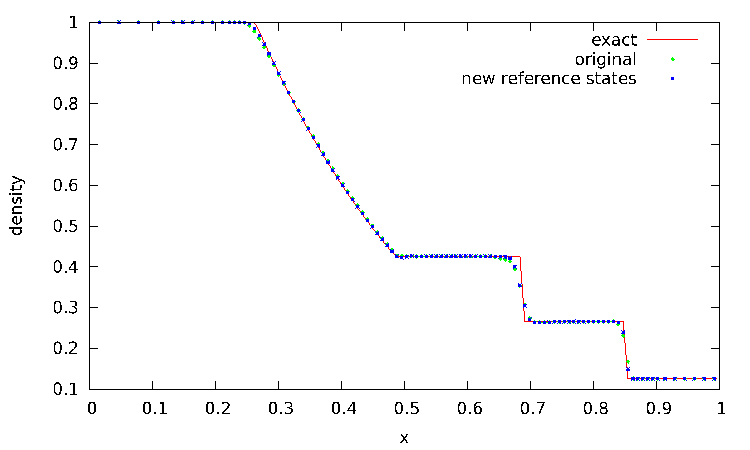
\includegraphics[scale=1.0]{reference}
  \caption{ \label{Fig:sod} Solution to Sod's problem with the original
    reference state and the new reference state, as compared to the
    exact solution.  We note that the new reference state shows a
    slightly sharper shock and contact, but also has a dip at the tail
    of the rarefaction.}
\end{figure}

\clearpage

%\begin{figure}
%  \centering
%  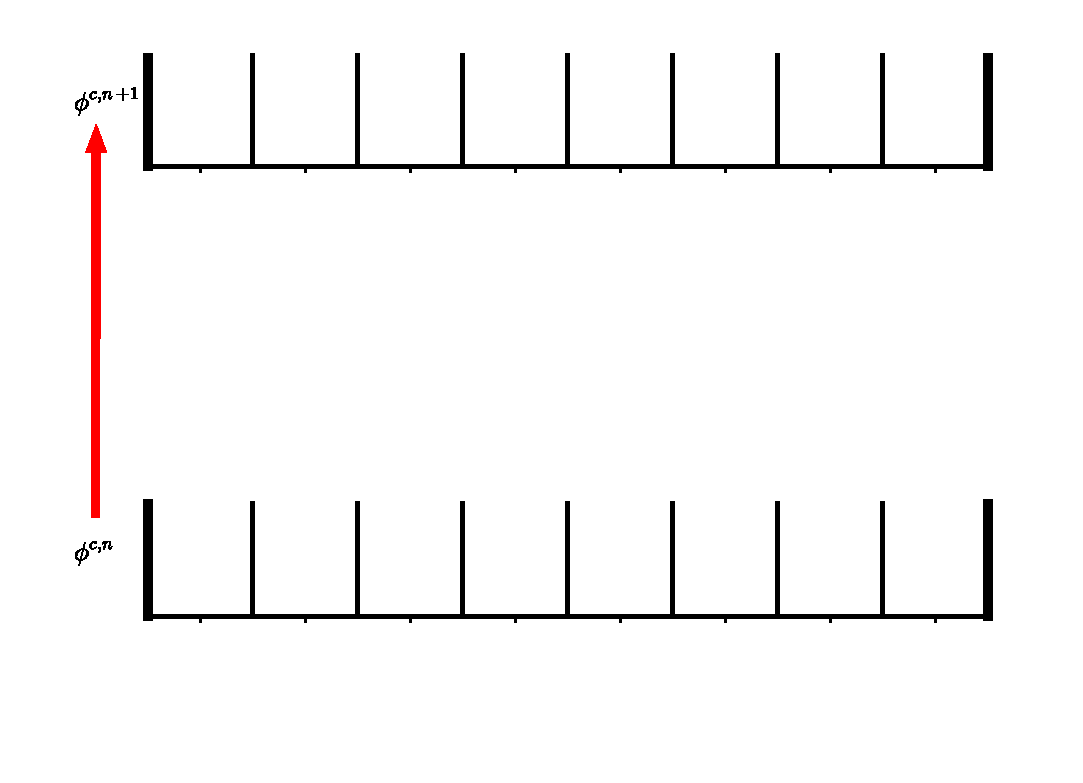
\includegraphics[width=3.1in]{nested2}\hspace{1em}
%  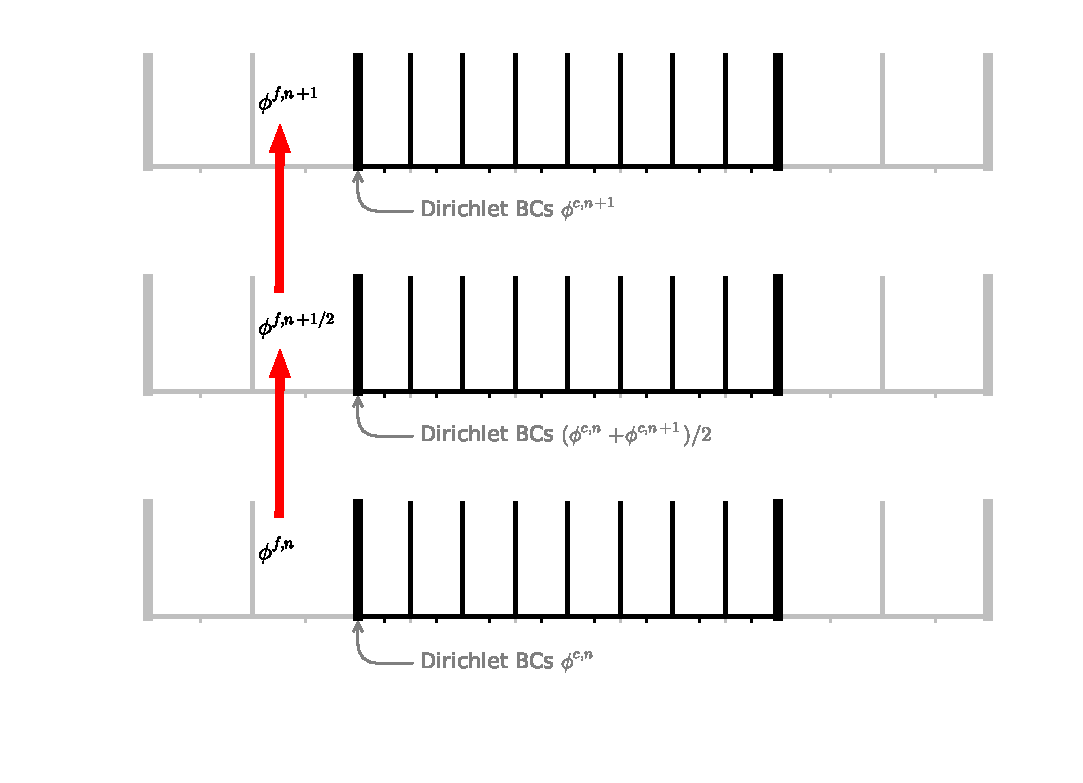
\includegraphics[width=3.1in]{nested3}
%  \caption{\label{fig:2levgrav} Schematic showing the solve for $\phi$ for a 2-level grid.}
%\end{figure}

\clearpage

\begin{figure}
  \centering
  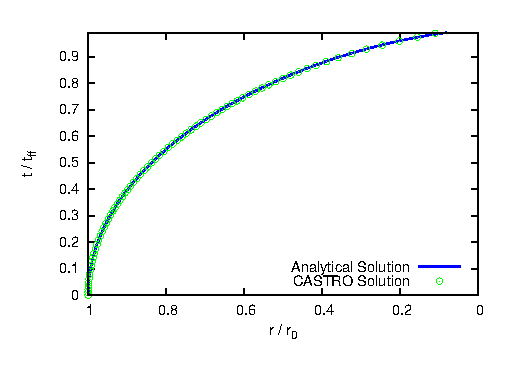
\includegraphics[scale=2.0]{freefall/plot_freefall}
  \caption{Time evolution of two initially stationary white dwarfs,
    mutually attracted to each other by the gravitational force. The
    horizontal axis gives the separation of the white dwarfs, scaled
    to the initial separation, and the vertical axis gives the elapsed
    time of the simulation, scaled to the total elapsed time
    necessarily. The solid curve shows the analytical result,
    calculated from Newtonian mechanics, and the circles show the
    samples from the time evolution with CASTRO. The agreement between
    theory and simulation is excellent, even for a simulation with
    modest resolution.}
  \label{Fig:Free Fall}
\end{figure}


\end{document}

